\chapter{Trainings- und Testdaten}
Zum Zeitpunkt, als diese Arbeit verfasst wurde, existierte noch keine Möglichkeit Echtdaten in einem
realistischen Szenario mit einem Mikrocontroller aufzunehmen, der über alle nötigen Sensoren verfügt.
Aus diesem Grund wurden Trainings- und Testdaten simulativ erfasst.
\newline
\newline
Zur Datenerfassung wurde wurde der Simulator CoppeliaSim verwendet, der zur Simulation von Robotik in Fabrikumgebungen entwickelt wurde \cite{coppeliaSim}.
Mit diesem Simulator wurden verschiedene Routen aus Fließbändern simuliert und dabei verschiedene Sensorwerte erfasst.
Diese wurden in einem Vorverarbeitungsschritt gefiltert und mit Sensordaten ergänzt, die in CoppeliaSim nicht verfügbar sind.
Zuletzt wurden Features extrahiert und die resultierende Datenmenge in Trainings-, Validations- und Testdaten unterteilt.

\section{Simulierte Sensordaten}
Insgesamt wurden vier Routen über 20 Zyklen erfasst, jeweils zwei mal erfasst.
Einmal für Testdaten und einmal für Trainingsdaten, wobei die letzten fünf Zyklen der
Trainingsdaten als Validationsmenge genutzt wird, die außerdem zur Feature-Auswahl genutzt wird.
Dabei wurden alle 50 ms die xyz-, Koordinaten, Beschleunigung und Gyroskopdaten erfasst, sowie Lichtintensität und Metadaten.
Zu den Metadaten gehören Zeitstempel, Beschriftung des Routenabschnitts und Beschriftung des derzeitigen Zyklusses.
Ein Zyklus ist der vollständige Umlauf einer Route.
\newline
\newline
Abbildung \ref{fig:simple_square_labeled} zeigt eine der vier Routen \glqq simple\_square\grqq.
Jede Route ist mit Markierungen für Zyklen und Standorte ausgestattet.
Die Zyklusmarkierung wird genutzt, um die die Datensätze mit deren derzeitigen Zyklus zu beschriften.
Jedes mal, wenn die Sensorenbox diese Markierung überschreitet, wird der Zähler für den Zyklus inkrementiert.
Die Standortmarkierung wird genutzt, um die Datensätze mit dem derzeitigen Routenabschnitt zu beschriften.
Jedes mal, wenn die Sensorenbox diese Markierung überschreitet, wird der derzeitige Wert für Routenabschnitt auf den Wert der Markierung gesetzt.
Dabei werden alle aufgenommenen Datensätze immer mit dem derzeitigen Wert für den Routenabschnitt markiert.
\begin{figure}[h!]
    \centering
    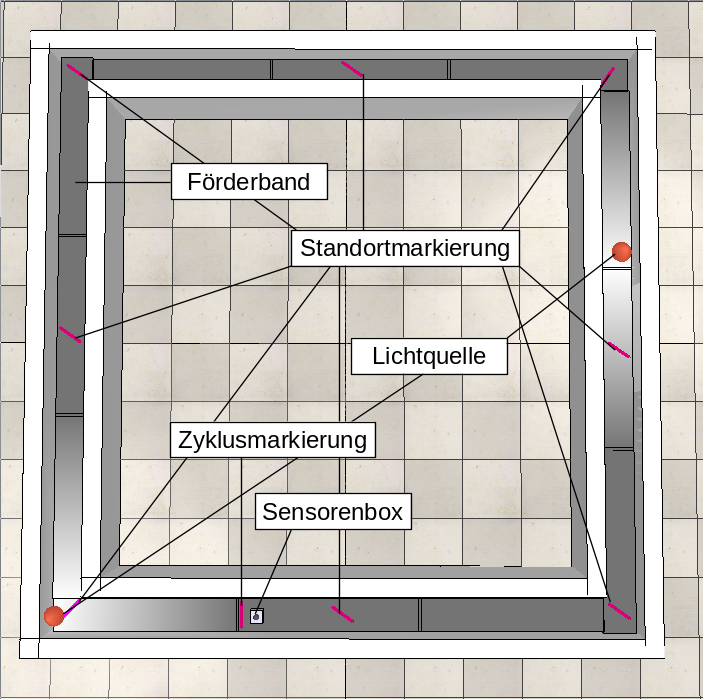
\includegraphics[width=\linewidth]{images/simple_square_labeled.png}
    \caption{Modell der Route \glqq simple\_square\grqq\ in CoppeliaSim mit Beschriftungen.}
    \label{fig:simple_square_labeled}
\end{figure}
\newline
\newline
Neben \glqq simple\_square \grqq\ gibt es noch drei weitere Routen (siehe Abbildungen \ref{fig:long_rectangle}, \ref{fig:rectangle_with_ramp} und \ref{fig:many_corners}).
Die Route \glqq long\_rectangle \grqq\ weist lange Pfade mit wenig Änderungen auf.
Die Route \glqq rectangle\_with\_ramp \grqq\ besitzt zusätzlich zwei Rampen, wodurch Höhenunterschiede simuliert werden.
Die Route \glqq many\_corners \grqq\ ist sehr komplex und hat viele verschiedene Standorte.
Die Förderbänder können verschiedene Geschwindigkeiten haben mit sowohl abrupten Übergangen, als auch fließenden Übergängen zueinander.
\newline
\newline
Je nach Enkodierungsart (siehe Kapitel \ref{sec:model_location_encoding}) müssen die Knoten und Kanten, dieses zyklischen Graphen, als Standorte enkodiert werden.
Als Knoten wird die Menge der Datensätze bezeichnet, die sich in einem Umkreis des ersten Datensatzes befinden, der mit einem Standort beschriftet ist,
d. h. Datensätze mit der gleichen Standortbeschriftung, die sich nicht im Umkreis des initialen Datensatzes befinden, gelten nicht als dieser Standort.
Die Knoten werden mit dem Wert der Standortbeschriftung beschriftet.
Die übrigen Datensätze werden entweder als unbekannten Standort beschriftet oder erhalten einen diskreten Standortwert, der die Beziehung der Kante zwischen zwei Knoten enkodiert.
\section{Künstlichen Sensordaten}
\begin{itemize}
    \item Motivation: Warum ist das nötig?
    \item Sag das vereinfachte Modelle genutzt werden mit bestimmten Annahmen
\end{itemize}

\subsection{Magnetfeld}
\begin{itemize}
    \item Welchen Sensor spiegelt das wieder?
    \item Wie funktioniert das Modell?
    \item Was und Wie wurden Daten ergänzt?
\end{itemize}

\subsection{Temperatur}
\begin{itemize}
    \item Welchen Sensor spiegelt das wieder?
    \item Wie funktioniert das Modell?
    \item Was und Wie wurden Daten ergänzt?
\end{itemize}

\subsection{Lautstärke}
\begin{itemize}
    \item Welchen Sensor spiegelt das wieder?
    \item Wie funktioniert das Modell?
    \item Was und Wie wurden Daten ergänzt?
\end{itemize}

\subsection{WLAN Zugangspunkte}
\begin{itemize}
    \item Welchen Sensor spiegelt das wieder?
    \item Wie funktioniert das Modell?
    \item Was und Wie wurden Daten ergänzt?
\end{itemize}
\section{Simulation von Interrupts}
Die Simulationsdaten, die mit CoppeliaSim aufgenommen wurden, enthalten alle 50 ms Einträge für die aufgenommen Sensoren.
Unter realen Bedingungen wäre solch eine Abtastrate aber nicht mit den Limitierungen der Batterielaufzeit zu vereinbaren.
Aus diesem Grund führen in solchen Systemen Sensoren \textit{Interrupts} aus, wenn eine signifikante Änderung festgestellt oder ein Schwellenwert überschritten wurde.
Interrupts sind Benachrichtigungen an die CPU, dass der Sensor ausgelesen werden, wodurch die CPU in der Zwischenzeit schlafen und somit Energie preservieren kann.
\newline
\newline
Um dieses Verhalten nachzustellen werden diese Interrupts simuliert, wodurch die Datenmenge gefiltert wird.
In dieser Arbeit wird die Änderung zu dem letzten Interrupt eines Sensors modelliert,
d. h. jeder Sensor merkt sich seinen Sensorwert, wenn es einen Interrupt auslöst
und führt das nächste mal nur einen Interrupt aus, wenn sich der Sensorwert um einen bestimmten Prozentsatz zu dem gemerkten Sensorwert unterscheidet.
\newline
\newline
Dadurch wird einerseits ein realistischeres Szenario dargestellt,
denn von einer Sensorenbox die still steht würde auch keine Aktivität erwartet werden.
Andererseits verringert sich die Datenmenge, wodurch die Trainingszeit verringert wird.
\newline
\newline
Unterschieden werden drei Ansätze, um Interrupts zu erzeugen.
Der erste Ansatz vergleicht den Betrag der Differenz mit einem festen Schwellenwert.
Der zweite Ansatz erfordert, dass die Änderung einen Prozentsatz des vorherigen Wertes ausmacht.
Der dritte Ansatz erfordert nur eine Änderung.
\newline
\newline
Die verwendeten Ansätze und Schwellenwerte sind Tabelle \ref{tab:interrupt_values} zu entnehmen.
Für Sensorwerte des Accelerometers und Gyroskops, sowie des Magnetfeldsensors wurde der erste Ansatz verwendet,
da signifikante Änderungswerte nicht relativ zu dem vorherigen Sensorwert sind, sondern lediglich eine absolute Änderung erzeugen.
Für Sensorwerte des Temperatur-, Licht- und Geräuschsensors wurde der zweite Ansatz verwendet,
da diese ein allgegenwärtiges Rauschen aufnehmen, das je nach Umgebung varrieren kann.
Für die WLAN-Zugangspunkte wird der dritte Ansatz verwendet, da die Sensorwerte binär sind.
\begin{table}[h!]
    \centering
    \begin{tabular}{ | l | c | c | c | }
        \hline
        Sensordaten & Fester Schwellenwert & Variabler Schwellenwert & Änderung \\\hline
        Accelerometer & 0.1 & - & - \\\hline
        Gyroskop & 0.1 & - & - \\\hline
        Magnetfeld & 8 & - & - \\\hline
        Temperatur & - & 0.12 & - \\\hline
        Licht & - & 0.12 & - \\\hline
        Geräusch & - & 0.16 & - \\\hline
        WLAN-Zugangspunkte & - & - & 1 \\\hline
    \end{tabular}
    \caption{Schwellenwerte der simulierten Interrupts.}
    \label{tab:interrupt_values}
\end{table}


\section{Feature-Extrahierung}
Die Feature-Extrahierung ist der Prozess, in dem Feature aus den Rohdaten der Datenmenge extrahiert werden.
In dieser Arbeit findet dieser Schritt nach der Filterung durch künstliche Interrupts statt.
Feature sind berechnete Attribute und Eigenschaften von einem oder mehreren Sensorwerten der Rohdaten.
\newline
\newline
Durch die Feature-Extrahierung müssen die ML-Modelle diese Features nicht selbständig lernen, sondern lediglich darauf abstrahieren.
Dies erleichtert das Training, kann aber gerade für tiefe NN die Generalisierungsfähigkeit einschränken,
wenn die Features nicht manuell konstruiert wurden \cite{seide2011feature}.
Einerseits benötigt aber der Entscheidungsbaum ML-Modell einen solchen Prozess,
da Features das Rauschen der Rohdaten verringern und dadurch eine Partitionierung vereinfachen.
Andererseits kann das FFNN durch die Limitierungen der Hardware möglicherweise nicht groß genug sein, um diese Features zu erlernen.
\newline
\newline
Mian hat in seiner Arbeit ein Datenfenster verwendet, um die Sensorwerte zu glätten \cite{naveedThesis}.
Als Datenfenster werden die letzten $N$ Einträge der Sensordaten bezeichnet, wobei $N$ die Fenstergröße ist.
Mian auch eine hohe Abtastrate verwendet, wodurch die Unterschiede zu hintereinander liegenden Datensätzen gering ist und Rauschen eine große Auswirkung hat.
Durch die künstlichen Interrupts werden nur Datensätze verwendet, die signifikante Änderungen enthalten,
wodurch große Datenfenster in dieser Arbeit nicht benötigt werden.
In der Praxis hat sich dennoch ein Datenfenster als sinnvoll erwiesen, da dadurch mehr Features konstruiert werden können,
die eine bessere Generalisierung ermöglichen.
Allerdings hat sich gezeigt, dass ein zu großes Datenfenster durch die im Mittel geringe Abtastrate, die Klassifizierungsgenauigkeit verringert.
Dies kann durch die künstlichen Interrupts begründet werden, da in einem großen Datenfenster dann
noch Datensätze enthalten sind, die zur Erkennung eines Standorts nicht mehr relevant sind.
\newline
\newline
Tabelle \ref{tab:all_features} listet alle verwendeten Features auf.
Zunächst werden aus jeden Sensor die gleiche Menge von Features extrahiert, sofern der Sensor dies erlaubt.
Aus den Datenfenstern der Sensordaten werden die Standardabweichung, Minimum, Maximum und der Durchschnitt für jeden Sensor berechnet.
Zusätzlich wird der momentane Wert jedes Sensors als Feature verwendet.
Da die Werte des Accelerometers und Gyroskops abhängig von der Ausrichtung der Sensorenbox ist,
wird von denen nur der Betrag der Summe der x-, y- und z-Komponenten verwendet.
Für die Detektionsdaten der WLAN-Zugangspunkte erschien die Standardabweichung, Minimum, Maximum und Durchschnitt nicht sinnvoll, da die Daten nur binäre Werte annehmen.
\begin{table}[h!]
    \hspace{-0.65cm}
    \begin{tabular}{ | l | c | c | c | c | c | }
        \hline
        Sensordaten & Standardabweichung & Minimum & Maximum & Durchschnitt & Wert \\\hline
        Accelerometer & X & X & X & X & X \\\hline
        Gyroskop & X & X & X & X & X \\\hline
        Magnetfeld & X & X & X & X & X \\\hline
        Temperatur & X & X & X & X & X \\\hline
        Licht & X & X & X & X & X \\\hline
        Geräusch & X & X & X & X & X \\\hline
        WLAN-Zugangspunkte & - & - & - & - & X \\\hline
        Letzter Standort & - & - & - & - & X \\\hline
        Zeit & X & - & - & - & - \\\hline
    \end{tabular}
    \caption{Extrahierte Features aus verfügbaren Sensordaten.}
    \label{tab:all_features}
\end{table}
\newline
\newline
Daneben wurden noch drei weitere Features aus den Metadaten extrahiert.
Das erste Feature ist der zuletzt bestimmte Standort des ML-Modells.
Das zweite Feature ist der zuletzt bestimmte Standort des ML-Modells, dass nicht als unbekannter Standort gilt und nicht der aktuelle Standort ist.
Mian hat ein Feature für jeden zu klassifizierenden Standort als Eingabe benutzt, dass auf eins gesetzt wird, wenn es erkannt wurde und ansonsten exponentiell abfällt \cite{naveedThesis}.
In dieser Arbeit wurde sich dagegen entschieden, da dies schlecht skaliert mit der steigenden Anzahl von zu klassifizierenden Standorten
und eine Abhängigkeit von dem zuletzt bestimmten Standort für die Robustheit vermieden werden sollte.
Das dritte Feature ist die Standardweichung über die Zeit des Datenfensters.
Alle anderen Features sind Zeitunabhängig, da sie sich auf Zeitunabhängige Sensorwerte im Datenfenster beziehen.
\newline
\newline
Die Signifikanz der einzelnen Features ist abhängig von der Einsatzumgebung, weshalb in Kapitel \ref{sec:model_training}
ein Feature-Auswahl Schritt in dem Trainingsprozess vorgeschlagen wurde, um die Anzahl der Features zu verringern.
Dabei wird die Signifikanz oder Wichtigkeit über die Permutationswichtigkeit bestimmt.
Aus diesem Grund muss individuell für jedes Einsatzgebiet abgewogen werden, welche Sensoren und Features am meisten Nutzen bringen
im Vergleich zu deren Kosten und Energieverbrauch.

\section{Synthetische Daten}
Es kann passieren, dass Sensoren über die Zeit kaputt gehen oder vorübergehend gestört werden.
Ist die Abhängigkeit des ML-Modells zu groß zu diesen Sensoren, dann wird die Klassifizierungsfähigkeit des ML-Modells stark eingeschränkt, wenn dieser Fall eintritt.
Um die ML-Modelle robust gegenüber diesen Szenarien zu machen, werden synthetische Daten auf Basis existierenden Daten erzeugt, die zusätzlich im Training benutzt werden.
\newline
\newline
Mögliche Fehler der Sensoren sind temporärer oder permanenter Ausfall oder leichte Abweichungen zum Originalwert.
Zudem können Standorte nicht erfasst werden, weil kein Interrupt ausgelöst wurde als die Sensorenbox sich an diesem Standort befand
oder die Sensorbox hat auf unbekannten Wege einen Standorte übersprungen.
\newline
\newline
Fehlerhafte Sensoren werden durch die Duplizierung von Routen dargestellt, in denen die Sensoren genullt werden bzw. ein zufälliges Rauschen addiert wird.
Verpasste Standorte werden zum einen durch permutierte duplizierte Routen dargestellt.
Zum anderen werden sie durch duplizierte Routen dargestellt, in denen der zuletzt besuchte nicht unbekannte Standort übersprungen wurde.
Um keinen Bias zu erzeugen, werden von den synthetischen Routen 10\% von jedem Standort zur Trainingsmenge hinzugefügt.
\section{Anomaliedaten}
\label{sec:data_anomalie}
Für Anomaliedaten werden die bekannten Routen modifiziert, indem Umleitungen eingebaut werden, die teilweise Standorte überspringen
und nicht in den Trainingsdaten vorhanden sind.
Dadurch wird ein Szenario simuliert, in der das Klassifizierungsverhalten von dem ML-Modell zur Standortbestimmung auf unbekannten Wegen beobachtet werden kann.
Aus den Klassifizierungsergebnissen des ML-Modells zur Standortbestimmung werden schließlich Features extrahiert,
die von dem ML-Modell zur Anomalieerkennung verwendet werden.
\begin{figure}[h!]
    \centering
    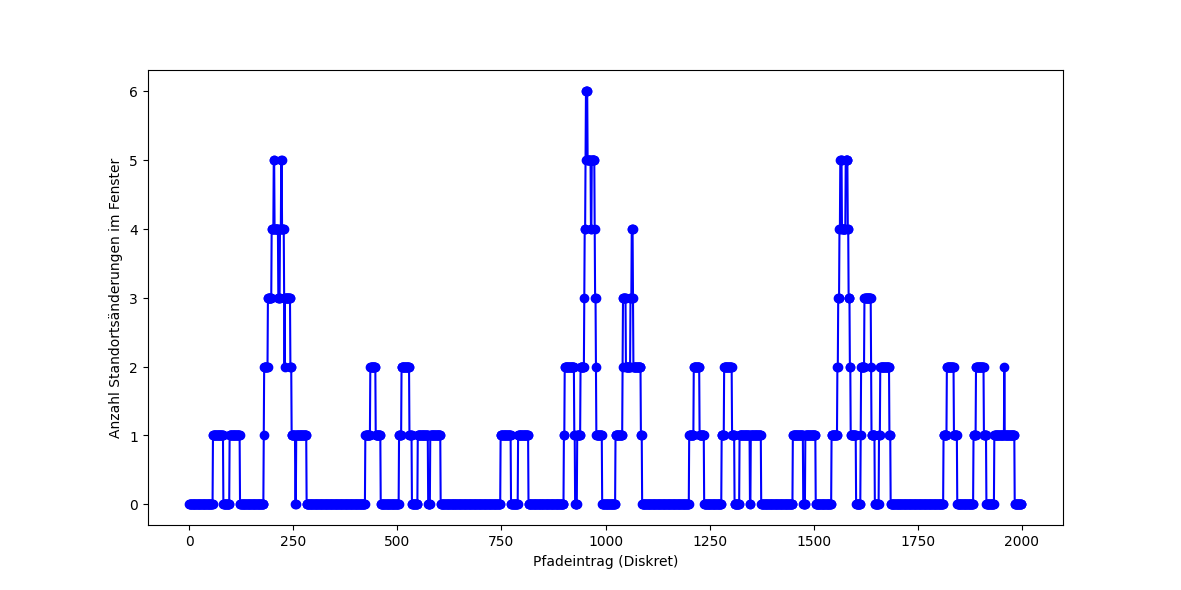
\includegraphics[width=\linewidth]{images/feature_window_location_changes.png}
    \caption{Ausschnitt der Anomalietestmenge mit den Standortänderungen in einem Datenfenster von 25.}
    \label{fig:window_location_changes}
\end{figure}
\newline
\newline
Wenn eine Anomalie vorliegt, wird erwartet, dass das ML-Modell unsicherer wird und stärker fluktuiert,
wodurch drei Features motiviert sind.
Das erste Feature ist abgeleitet aus der Anzahl der Standortänderungen.
Das Feature ist der Betrag der Differenz von den folgenden Komponenten.
Die erste Komponente ist die durchschnittliche Anzahl der Standortänderungen in einem Datenfenster.
Die zweite Komponente die durchschnittliche Anzahl der Standortänderungen, wenn keine Anomalie vorliegt.
Abbildung \ref{fig:window_location_changes} zeigt die akkumulierten Standortänderungen in einem Datenfenster von 25.
Bei den Pfadeinträgen bei ca. 250, 1000 und 1600 sind Extrema zu erkennen, die mit der Anomalie in dieser Testmenge übereinstimmen,
d. h. wenn eine Anomalie vorliegt wird häufiger der Standort geändert.
\newline
\newline
Das zweite Feature ist analog zu dem ersten Feature konstruiert.
Dieses nutzt ansatt der Anzahl der Standortänderungen die summierte Wahrscheinlichkeit der erkannten Standorte.
Das ML-Modell zur Standortbestimmung hat keine diskrete Ausgabe, sondern gibt einen Vektor von Wahrscheinlichkeiten aus,
der für jeden Standort die Klassifizierungswahrscheinlichkeit angibt.
Dabei gilt der klassifizierte Standort als der Eintrag im Vektor mit der höchsten Wahrscheinlichkeit.
Diese Wahrscheinlichkeit wird dann analog zu den Standortänderungen summiert.
Das dritte Feature ist die Standardabweichung der ersten fünf Einträge dieses Vektors, der absteigend sortiert ist.
Abbildung \ref{fig:window_confidence} zeigt die akkumulierte Standortwahrscheinlichkeit in einem Datenfenster von 25.
Bei den Pfadeinträgen bei ca. 250, 1000 und 1600 ist die akkumulierte Standortwahrscheinlichkeit deutlich geringer als läge keine Anomalie vor,
d. h. wenn eine Anomalie vorliegt, ist die Sicherheit für einen Standort geringer.
\begin{figure}[h!]
    \centering
    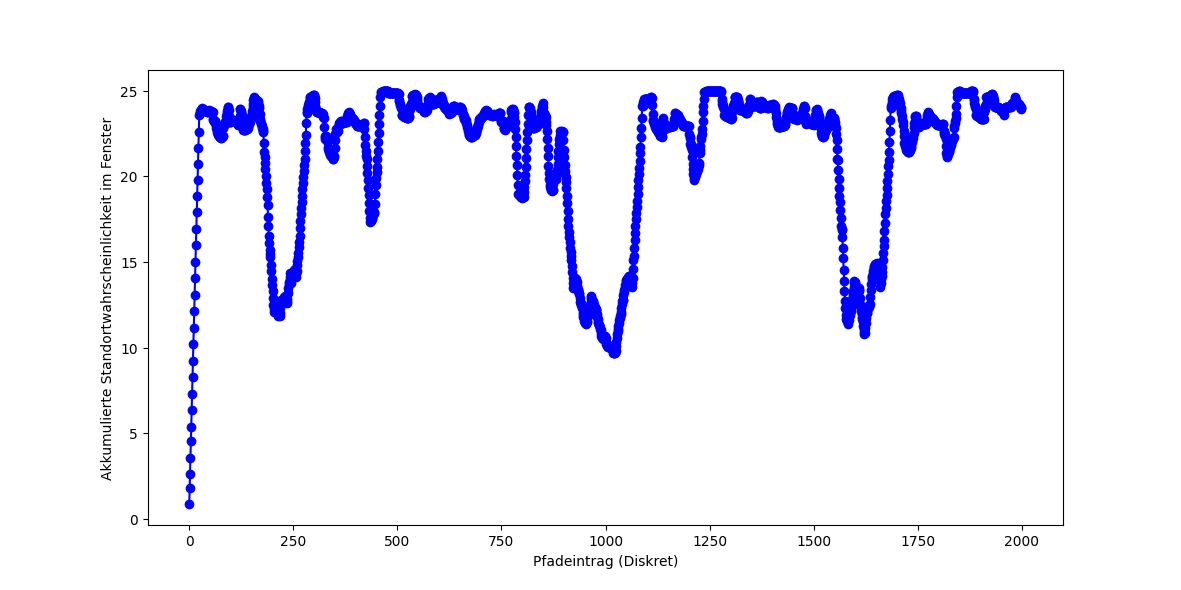
\includegraphics[width=\linewidth]{images/feature_window_confidence.png}
    \caption{Ausschnitt der Anomalietestmenge mit der akkumulierten Standortwahrscheinlichkeit in einem Datenfenster von 25.}
    \label{fig:window_confidence}
\end{figure}
\newline
\newline
Zusätzlich wird das Ergebnis des Modells auf Basis der Topologie als Feature verwendet.
Dieses Feature indiziert, dass das ML-Modell zur Standortbestimmung ein Fehler gemacht haben muss
oder dass tatsächlich eine Anomalie vorliegt, da die Topologie verletzt wurde.
\newline
\newline
Daneben wurde ebenfalls eine Rückwärtskante in Betracht gezogen,
da es wahrscheinlich ist, dass wenn zuvor eine Anomalie vorlag, danach immer noch eine Anomalie vorliegt.
Im Training wurden damit zwar sehr gute Ergebnisse erreicht,
in der Praxis war das Modell aber äquivalent zu dem \textit{Immer-Falsch} Modell.
